% Chapter 20. Hash chaining, and the one number you publish.
\documentclass[tikz,border=6pt]{standalone}
% Shared look for every TikZ figure in the book.
% Colours match book/preamble.tex exactly. Change both or neither.

\usepackage{tikz}
\usepackage{xcolor}
\usepackage{amsmath}
\IfFileExists{libertinus.sty}{\usepackage[mono=false]{libertinus}}{}
\IfFileExists{inconsolata.sty}{\usepackage[varqu,varl,scaled=0.95]{inconsolata}}{}

\usetikzlibrary{
  arrows.meta, positioning, calc, fit, backgrounds, shapes.geometric,
  shapes.misc, decorations.pathreplacing, decorations.pathmorphing,
  patterns, chains, matrix, shadows.blur
}

\definecolor{ink}{HTML}{15181D}
\definecolor{muted}{HTML}{5B6472}
\definecolor{rule}{HTML}{C9CED6}
\definecolor{wash}{HTML}{F4F5F7}
\definecolor{accent}{HTML}{0F5C8C}
\definecolor{accentsoft}{HTML}{E7F0F6}
\definecolor{warm}{HTML}{B4531A}
\definecolor{warmsoft}{HTML}{FBF0E7}
\definecolor{good}{HTML}{2C6E49}
\definecolor{goodsoft}{HTML}{E9F2EC}
\definecolor{danger}{HTML}{9B2226}
\definecolor{dangersoft}{HTML}{FAECEC}

\tikzset{
  font=\sffamily\small,
  >={Stealth[length=5pt, width=4pt]},
  %
  box/.style={
    draw=rule, line width=0.8pt, fill=wash, rounded corners=2pt,
    inner sep=7pt, align=center, text=ink, minimum height=9mm,
  },
  boxa/.style={box, draw=accent, fill=accentsoft},
  boxg/.style={box, draw=good,   fill=goodsoft},
  boxw/.style={box, draw=warm,   fill=warmsoft},
  boxd/.style={box, draw=danger, fill=dangersoft},
  %
  lane/.style={draw=rule, line width=0.7pt, fill=white, rounded corners=2pt,
               inner sep=6pt, align=center, minimum width=26mm},
  %
  flow/.style={draw=accent, line width=1.0pt, ->},
  flowback/.style={flow, densely dashed},
  flowmuted/.style={draw=muted, line width=0.8pt, ->},
  lifeline/.style={draw=rule, line width=0.7pt, densely dotted},
  %
  lbl/.style={font=\sffamily\scriptsize, text=muted, inner sep=2pt},
  lblink/.style={font=\sffamily\scriptsize, text=ink, inner sep=2pt},
  tag/.style={font=\ttfamily\scriptsize, text=accent, inner sep=2pt,
              fill=white, inner xsep=3pt},
  note/.style={font=\sffamily\scriptsize\itshape, text=muted, align=left},
  %
  band/.style={draw=none, rounded corners=1pt},
  tick/.style={draw=muted, line width=0.6pt},
}

% A horizontal timeline bar segment: \barseg{x0}{x1}{y}{colour}{label}
\newcommand{\barseg}[5]{%
  \fill[#4, rounded corners=1pt] (#1,#3-0.16) rectangle (#2,#3+0.16);
  \node[lbl, text=white, font=\sffamily\scriptsize\bfseries]
       at ({(#1+#2)/2},#3) {#5};
}

\begin{document}
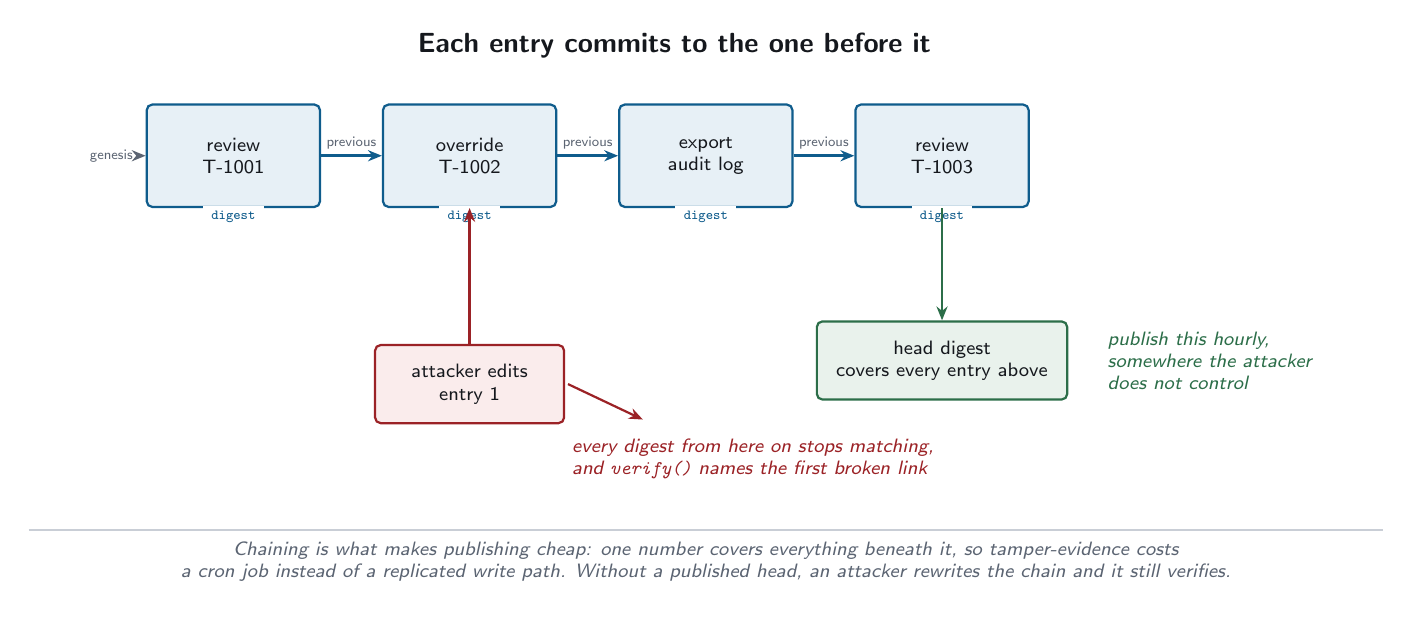
\begin{tikzpicture}[x=1cm, y=1cm]

  \node[lblink, font=\sffamily\bfseries] at (5.6,3.1) {Each entry commits to the one before it};

  \foreach \i/\x/\txt in {0/0.0/{review\\T-1001}, 1/3.0/{override\\T-1002},
                          2/6.0/{export\\audit log}, 3/9.0/{review\\T-1003}} {
    \node[boxa, minimum width=22mm, minimum height=13mm, font=\sffamily\scriptsize]
      (e\i) at (\x,1.7) {\txt};
    \node[tag, font=\ttfamily\tiny] at (\x,0.92) {digest};
  }

  \foreach \i/\j in {0/1, 1/2, 2/3} {
    \draw[flow] (e\i.east) -- node[lbl, above, font=\sffamily\tiny] {previous} (e\j.west);
  }

  \node[lbl, font=\sffamily\tiny] at (-1.55,1.7) {genesis};
  \draw[flowmuted] (-1.2,1.7) -- (e0.west);

  % the published head
  \node[boxg, minimum width=30mm, minimum height=9mm, font=\sffamily\scriptsize]
    (head) at (9.0,-0.9) {head digest\\{\scriptsize covers every entry above}};
  \draw[flow, draw=good] (e3.south) -- (head.north);
  \node[note, align=left, text=good] at (12.4,-0.9)
    {publish this hourly,\\somewhere the attacker\\does not control};

  % the tamper
  \node[boxd, minimum width=24mm, minimum height=8mm, font=\sffamily\scriptsize]
    (edit) at (3.0,-1.2) {attacker edits\\entry 1};
  \draw[flowmuted, draw=danger] (edit.north) -- (e1.south);
  \node[note, align=left, text=danger] at (6.6,-2.15)
    {every digest from here on stops matching,\\and \texttt{verify()} names the first
     broken link};
  \draw[flowmuted, draw=danger] (4.25,-1.2) -- (5.2,-1.65);

  \draw[rule, line width=0.7pt] (-2.6,-3.05) -- (14.6,-3.05);
  \node[note, align=center, text=muted] at (6.0,-3.45)
    {Chaining is what makes publishing cheap: one number covers everything
     beneath it, so tamper-evidence costs\\a cron job instead of a replicated
     write path. Without a published head, an attacker rewrites the chain and
     it still verifies.};

\end{tikzpicture}
\end{document}
